 \section{Actividad – Power BI} 
Para crear los informes en Power BI Desktop, primero debe conectarse a los datos y después darles forma. Después podrá guardar los informes en el formato de archivos de Power BI Desktop, que es la extensión .pbix. Y también va a poder compartirlos. Puede hacerlo como cualquier otro archivo, pero sin duda como va a aprovechar todo su potencial será si lo comparte desde el servicio de Power Bi.
\begin{itemize}
	\item Conectarse a datos: normalmente son varios orígenes de datos.
	\item Dar forma a dichos datos: mediante las consultas que crean modelos de datos precisos.
	\item Crear informes: usando modelos que otros pueden aprovechar, compartir y usar como punto de partida.\\
\end{itemize} 

Resultado (imagen) y la ruta del informe en el Portal de Power BI 
\begin{itemize}
	\item Resultado de publicar el reporte en el Power BI
	\begin{center}
	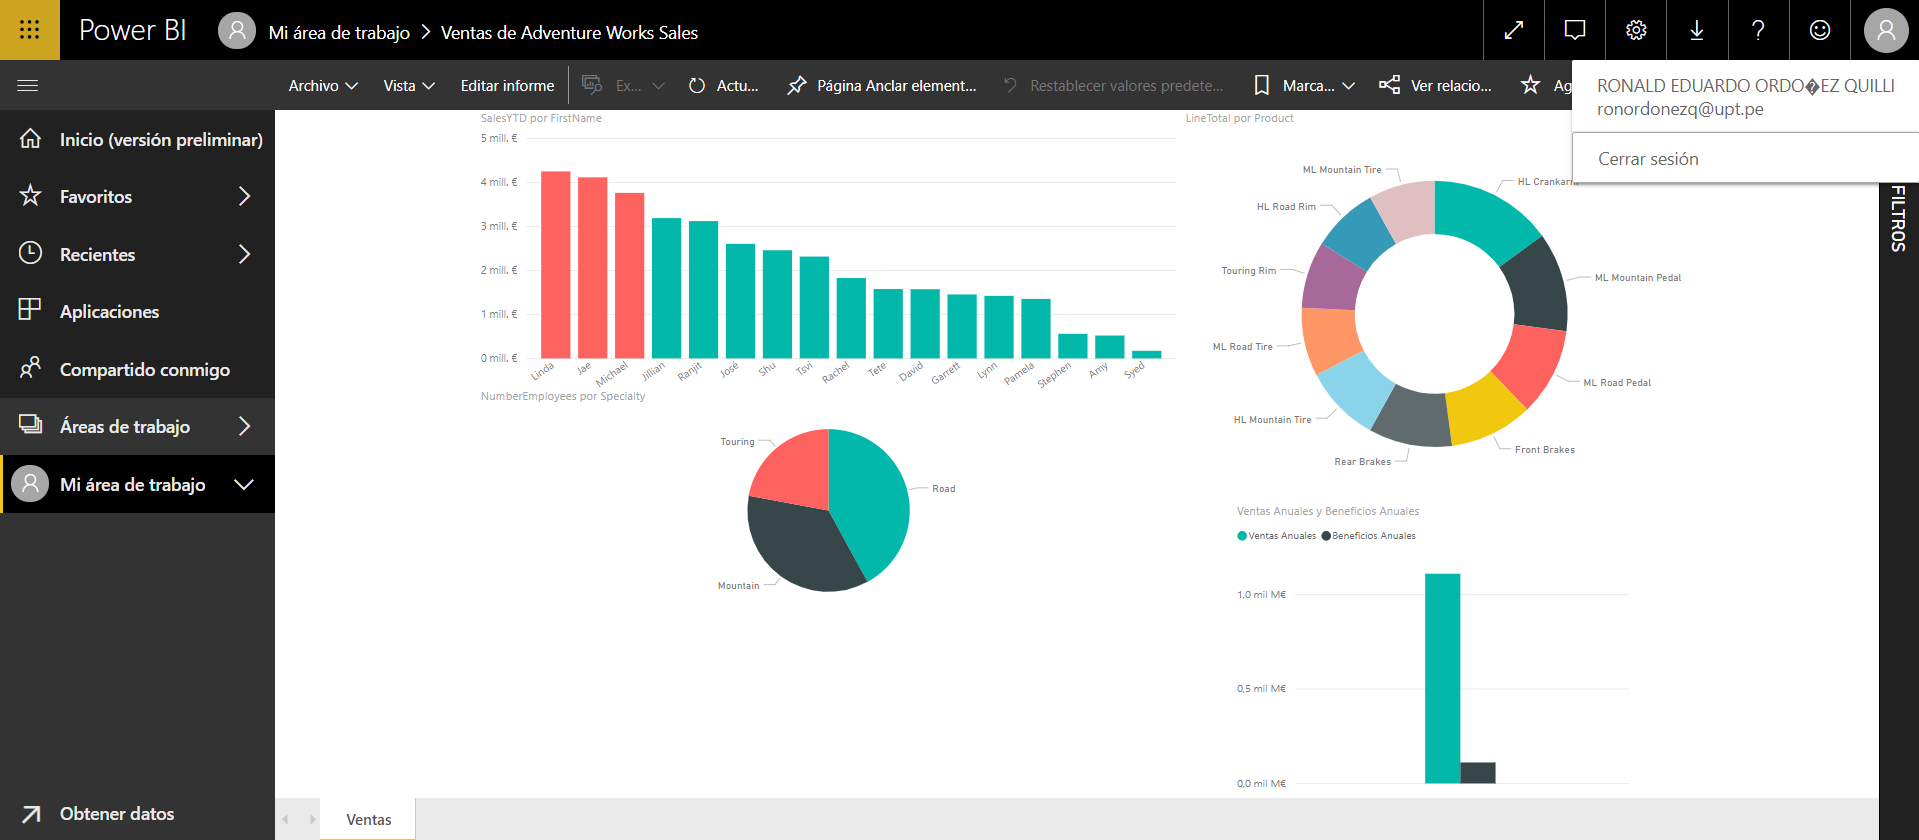
\includegraphics[width=16cm]{./Imagenes/img1} 
	\end{center}
Ruta del informe en el Power BI
\\
\url{https://app.powerbi.com/groups/me/reports/fbd481e5-ca85-44d3-9be4-41d98b574a21?ctid=b6b466ee-468d-4011-b9fc-fbdcf82ac90a} 
\end{itemize} 